\documentclass[11pt]{article}
\usepackage{appendix}
\usepackage{graphicx} 
\usepackage{setspace}
\usepackage{amsmath,float,verbatim,multicol}
\usepackage{array}
\usepackage{lscape}
\usepackage{hyperref}

\usepackage{amssymb}
\bibliographystyle{plainnat}
\usepackage[round]{natbib}
\usepackage{multirow}

\setlength{\textheight}{8.8in} \setlength{\textwidth}{6.3in}
\setlength{\oddsidemargin}{0.2in} \setlength{\topmargin}{-0.30in}
\setlength{\footnotesep}{10.0pt}

\newcommand{\ol}{\overline}



\renewcommand{\baselinestretch}{1.25}
\title{Solving an Infinitely-Lived Human Capital Accumulation Problem}
\author{ Trevor Gallen \\ Econ 64200 }
\date{Fall 2023}

\begin{document}
\bibliographystyle{myplainnat}
%\bibpunct{(}{)}{;}{a}{}{,}6868

\maketitle

This homework is the first part of a multi-part homework.  This homework starts us with a relatively simple deterministic lifecycle model and asks you to solve it in Matlab.\\

\textbf{Deliverables}
\begin{itemize}
\item You should have a word/\LaTeX document that has three sections: 
\begin{enumerate}
\item Discusses the model and answers the questions I pose throughout.
\item Contains the tables and figures you will produce.
\item Contains a discussion of your programming choices if you had to make any.
\end{enumerate}
\item You should have a Matlab file or set of files (zipped) that contain \textbf{all} your programs and raw data.  There should be a file called ``Main.M" that produces everything I need in one click.
\end{itemize}


\section{Model}
Infinitely-lived households start each period with human capital endowment $h_t$, and have period utility over consumption $c_t$.  They have one unit of time each period, which they use to either study $i_t$ or work $L_t$ . If they study, their human capital for next period grows, while if they work, consumption increases.  Households do not have access to savings technology.  They maximize the net present value of utility discounted at a rate $0<\beta<1$:
$$\sum_{t=0}^\infty \log(c_t)$$
subject to the law of motion of human capital:
$$h_{t+1}=(1-\delta)h_t+i_t$$
And their budget constraint:
$$c_t=h_tL_t$$

\ \\
\textbf{Question 1a:} Write out the household's Bellman equation subject to both constraints, with Lagrange multipliers $\lambda_{h}$,  $\lambda_{bc}$, $\lambda_{time}$ for the budget constraint, law of motion, and time Lagrange multipliers respectively. Don't plug in, keep all the equations!\footnote{I recognize plugging in is easier in this case, this is useful for practice in more complex problems, and for setting your mind straight on how to solve this sort of problem!}\\
\ \\
\textbf{Suggested Sol}: Should look something like:
$$V(h)=\underset{c,i,L,h'}{\max}\left\{\log(c_t)+\beta V(h')\right\}$$
s.t.
$$h_{t+1}=(1-\delta)h_t+Ai_t^\gamma \ \ \ \ (\lambda_h)$$
$$c_t=h_tL_t\ \ \ \ (\lambda_{bc})$$
$$L_t+i_t=1\ \ \ \ (\lambda_{time})$$

\ \\
\textbf{Question 1b:} Take first order conditions with respect to $c$, $i$, $L$, and $h'$, and find the Envelope condition for $h$ $\left(\frac{\partial V}{\partial h}=?\right)$.\\
 \ \\
\textbf{Suggested Sol}: Should look something like:\\
\ \\
\textbf{C:}\\
$$\frac{\partial \mathcal{L}}{\partial c}   =0\ \ \ \Rightarrow \ \ \ \frac{1}{c}  = \lambda_{bc}$$
\textbf{i:}\\
$$\frac{\partial \mathcal{L}}{\partial i}  =0\ \ \ \Rightarrow \ \ \ \gamma A i^{\gamma-1}\lambda_{h}=\lambda_{time}$$
\textbf{L:}\\
$$\frac{\partial \mathcal{L}}{\partial L}  =0\ \ \ \Rightarrow \ \ \ h\lambda_{bc}=\lambda_{time}$$
\textbf{h':}\\
$$\frac{\partial \mathcal{L}}{\partial h'}  =0\ \ \ \Rightarrow \ \ \ \beta V_{h'}=\lambda_h$$
\textbf{Envelope condition for $h$:}\\
$$\frac{\partial \mathcal{V}}{\partial h}  =(1-\delta)\lambda_h+\lambda_{bc}L$$
Advancing the Envelope condition one period, we get:
$$\beta \left((1-\delta)\lambda_h'+\lambda_{bc}'L'\right)=\lambda_h$$
Using the relationship between the multipliers:
$$\beta \left((1-\delta)\frac{1}{\gamma A i'^{\gamma-1}}\frac{h'}{c'}+\frac{L'}{c'}\right)=\frac{1}{\gamma A i'^{\gamma-1}}\frac{h}{c}$$

\textbf{Question 1c:} Using the elements from 1b, you should be able to derive an equation that looks like: $$\beta \left((1-\delta)\frac{1}{\gamma A i'^{\gamma-1}}\frac{h'}{c'}+\frac{L'}{c'}\right)=\frac{1}{\gamma A i'^{\gamma-1}}\frac{h}{c}$$
While this looks horrific at first glance, it's very simple to understand \emph{economically}.\footnote{For instance, when we take FOC's with respect to a standard labor/leisure tradeoff with preferences $u(c,L)=\log(c)+\psi\log(1-L)$ we get $u'(c)=\frac{1}{w}\frac{\psi}{1-L}$, which just says that the marginal benefit of one more unit of consumption, which is $1/c$, is equal to the marginal cost, which is the amount of time it took to earn that one unit $\frac{1}{w}$ multiplied by the marginal disutility of working that amount, $\frac{\psi}{1-L}$.}  Interpret each of the three pieces (breaking up the LHS into two additive pieces) economically. What does each mean?\\
 \ \\
\textbf{Suggested Sol}: Should look something like:\\
\begin{itemize}
\item $\frac{1}{\gamma A i'^{\gamma-1}}\frac{h}{c}$ this is the marginal cost another unit of human capital.  When I get one more unit of human capital, I spend $\frac{1}{\gamma A i'^{\gamma-1}}$ less units of time working.  This pays me that times $h$ less, which at a marginal utility of $\frac{1}{c}$, gives me the total cost.
\item $(1-\delta)\frac{1}{\gamma A i'^{\gamma-1}}\frac{h'}{c'}$ is (part of) the marginal benefit of investing time into more human capital!  If I get one more unit of human capital, I can reduce $i'$ by $(1-\delta)$, which increases $L$ by that amount.  Multiplying $L$ by $h$ gives me $(1-\delta)\frac{1}{\gamma A i'^{\gamma-1}}h$ more units of consumption, which at marginal utility $\frac{1}{c'}$ gives me my discounted reward $\beta\frac{1}{\frac{1}{\gamma A i'^{\gamma-1}}}\frac{(1-\delta)h'}{c'}$ as a marginal benefit.
\item But higher $h$ doesn't just help me with less investment in the future, it also increases my wage, which benefits me by $L$, again multiplied by the marginal utility of consumption gives $\frac{L'}{c'}$.
\end{itemize}

\clearpage
\section{Basic Matlab}
Now, let the following numerical assumptions hold:
\begin{table}[ht!]
\centering
\begin{tabular}{lcc}
\hline
\hline
\multicolumn{3}{c}{Table 1: Calibration}\\
\hline
Concept & Parameter & Value \\ 
Discount factor & $\beta$ & 0.95\\
Ability to accumulate human capital: $A$ &  & 1\\
Human capital depreciation rate: $\delta$ &  & 0.05\\
Decreasing returns to human capital investment: $\gamma$ &  & 0.6\\
\hline
\hline
\end{tabular}
\end{table}

\textbf{Question 2:} Write a Matlab program that takes in the parameterization of Table 1 and uses value function iteration to solve the agent's problem.  I suggest plugging in the constraints and writing your problem as a function of choosing $i$, but solve it how you want.\\
\ \\
\textbf{Suggested Sol}: See Main\_Hwk1.m \\

\textbf{Question 3:} Plot the policy function for $i$ as a function of $h$.  What is the steady state value of $h$?\\
\ \\
\textbf{Suggested Sol}: \\
Letting $i^*(h)$ be the interpolated policy function we solved for, to find the steady-state human capital level, I found the zero of the function:
$$(1-\delta)h+Ai^*(h)^\gamma-h=0$$
Which is the change in human capital (when it is zero, we're at steady state).

\begin{figure}[ht!]
\centering
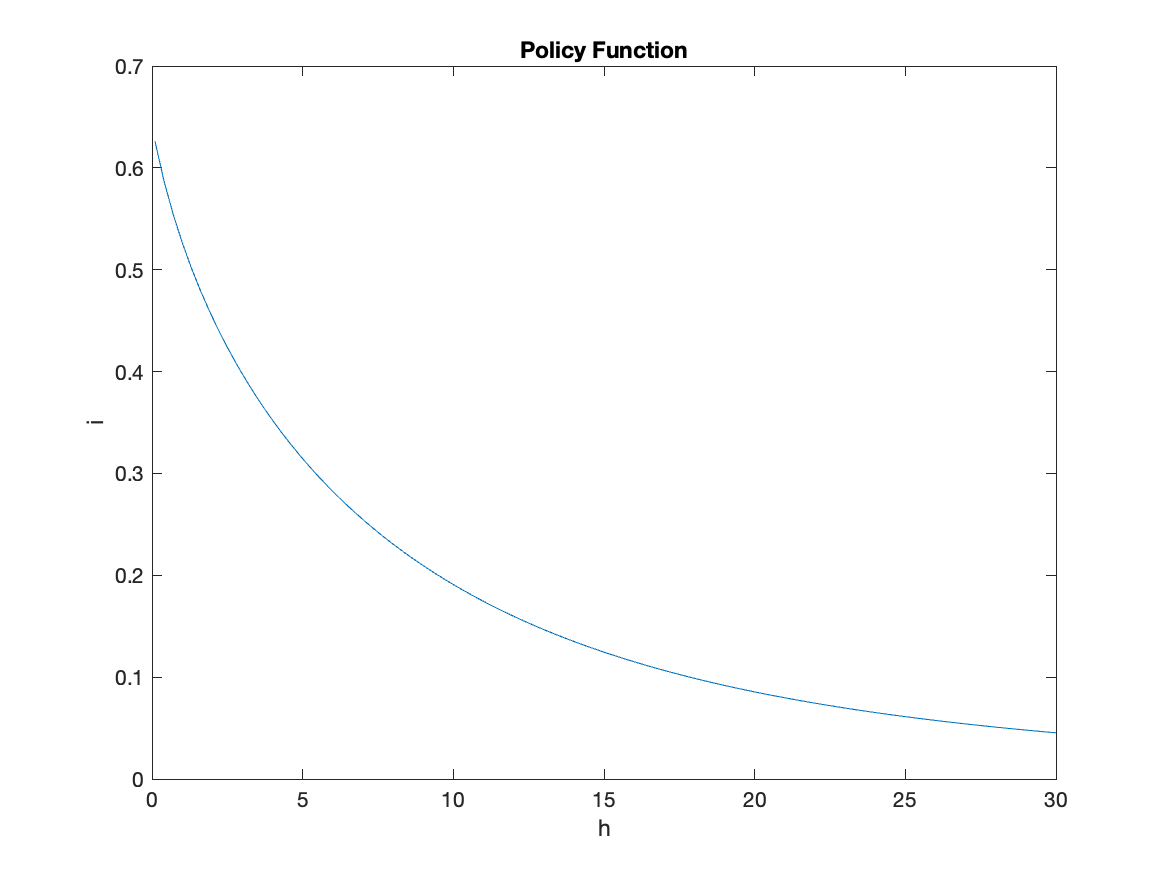
\includegraphics[scale=0.5]{Fig1.png}
\caption{This is the policy function for investment $(i)$ as a function of the state variable (human capital entering the period $(h)$.)}
\end{figure}

\clearpage
\textbf{Question 4:} Use the policy function for $i$ to simulate the evolution of human capital levels over time for $h_0=1$ and $h_0=10$ for 40 periods.  Plot your results.\\
\ \\
\textbf{Suggested Sol}: \\
\begin{figure}[ht!]
\centering
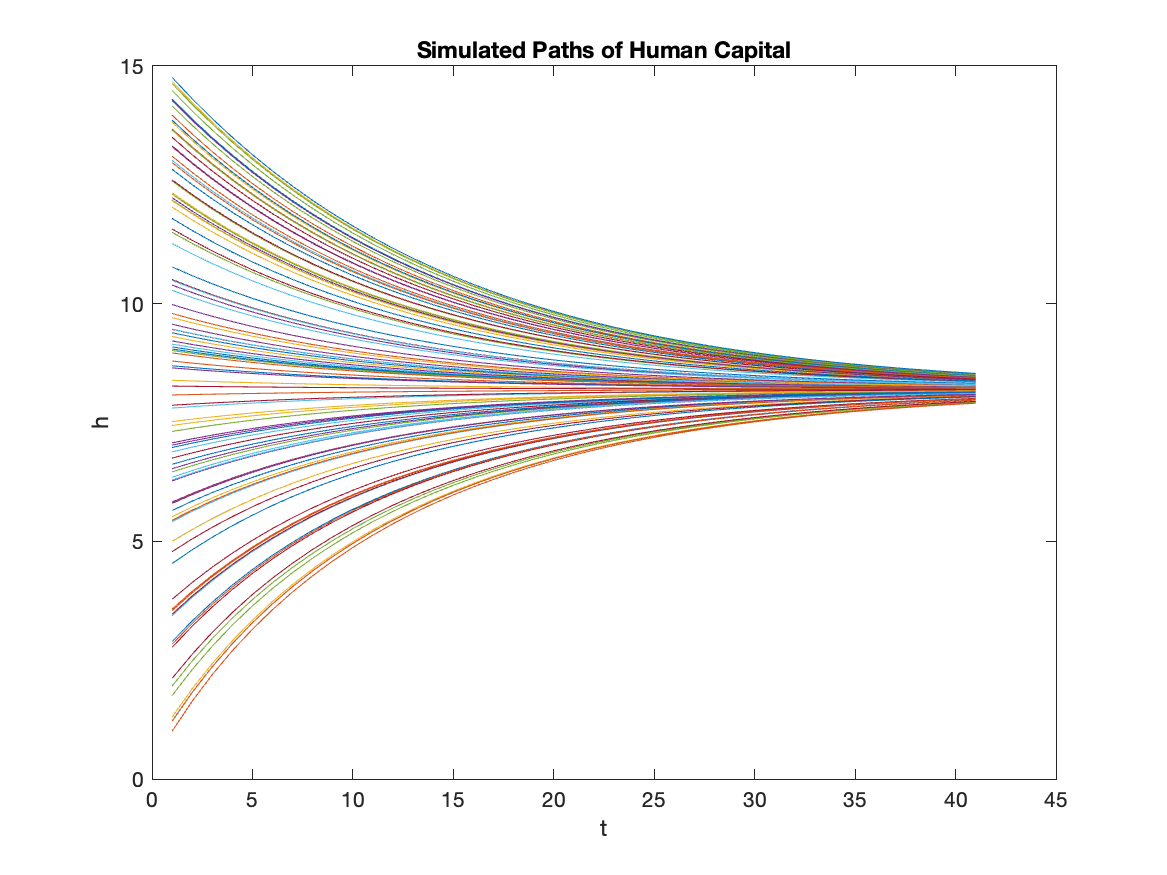
\includegraphics[scale=0.5]{Fig2.png}
\caption{This is a simulation of the evolution of human capital for 100 individuals with random initial human capitals.}
\end{figure}

\end{document}





